


\begin{frame}[fragile]
\frametitle{ViennaGrid User API}
 \begin{block}{User API Design Goals}
  \begin{itemize}
   \item STL-style, reuse conventions
   \item Allow index-based traversal
   \item Avoid common C++ pitfalls (e.g.~template member functions)
  \end{itemize}

  \begin{lstlisting}[basicstyle=\scriptsize\ttfamily,escapechar=@]
  //iteration over all vertices in the domain:
  typedef result_of::ncell_range<@\color{red}DomainType@, @\color{red}0@>::type  VertexRange;
  typedef result_of::iterator<VertexRange>::type       VertexIterator;
  
  VertexRange vertices = ncells<@\color{red}0@>(@\color{red}domain@);
  for (VertexIterator it  = vertices.begin();
                      it != vertices.end();
                    ++it)
  {
    // do something with each vertex here
  }
  \end{lstlisting} 

   \begin{itemize}
    \item \emph{Ranges} provide iterators over $n$-cells
    \item Extendible
   \end{itemize}
 \end{block}
 \vspace*{0.45cm}
\end{frame}


\begin{frame}[fragile]
\frametitle{ViennaGrid User API}
 \begin{block}{User API Design Goals}
  \begin{itemize}
   \item STL-style, reuse conventions
   \item Allow index-based traversal
   \item Avoid common C++ pitfalls (e.g.~template member functions)
  \end{itemize}

  \begin{lstlisting}[basicstyle=\scriptsize\ttfamily,escapechar=@]
  //iteration over all vertices in the domain:
  
  for (std::size_t i = 0; i < ncells<@\color{red}0@>(@\color{red}domain@).size(); ++i)
  {
    // do something with ncells<0>(domain)[i] here
  }
  \end{lstlisting} 

   \begin{itemize}
    \item OpenMP friendly
    \item \lstinline|.size()| sometimes known at compiletime!
   \end{itemize}
 \end{block}
 \vspace*{1.75cm}
\end{frame}

 
\begin{frame}[fragile]
\frametitle{ViennaGrid User API}
 \begin{block}{User API Design Goals}
  \begin{itemize}
   \item Boundary iteration: $k < n$
   \item Coboundary iteration: $k > n$
  \end{itemize}
  
  \begin{flushright}
   \vspace*{-2cm}
   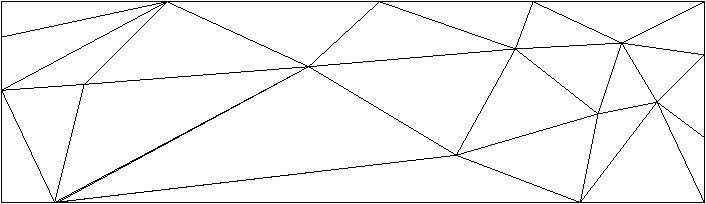
\includegraphics[width=0.5\textwidth]{figures/mesh.pdf}
  \end{flushright}


  \begin{lstlisting}[basicstyle=\scriptsize\ttfamily,escapechar=@]
  //iteration over all triangles of a vertex
  typedef result_of::ncell_range<@\color{red}VertexType@, @\color{red}2@>::type  TriangleRange;
  typedef result_of::iterator<TriangleRange>::type     TriangleIterator;
  
  TriangleRange triangles = ncells<@\color{red}2@>(@\color{red}vertex, domain@);
  for (TriangleIterator it  = triangles.begin();
                        it != triangles.end();
                      ++it)
  {
    // do something with each triangle here
  }
  \end{lstlisting} 

   \begin{itemize}
    \item Coboundary information not a-priori available in datastructure
    \item Built and cached at first request
   \end{itemize}
 \end{block}
 \vspace*{0.45cm}
\end{frame}
 


